%
% Documento: Ilustração
%
\chapter{ILUSTRAÇÕES}


A apresentação de quadros e tabelas está regida pelas Normas de Apresentação Tabular do Instituto Brasileiro de Geografia e Estatística.

\section{FIGURAS}

São desenhos, fotografias, organogramas, esquemas etc. com os respectivos títulos precedidos da palavra Figura e do número de ordem em algarismo arábico. Conforme ilustra a Figura \ref{fig:abnt}.

\begin{figure}[H]
    \centering
    
	\vspace*{0,2cm}
    
\includegraphics[width=0.5\textwidth]{./04-figuras/navegar_abnt}
    \caption{Exemplo de figura}
    \label{fig:ilustfig}
\end{figure}
\vspace*{-1,5cm}
{\raggedright \fonte{Disponível em: <https://www.gazetadopovo.com.br/abntemfoco>. Acesso em: 24 de jan. de 2015.}}\\


\begin{figure}[H]
    \centering
    
	\vspace*{0,2cm}
    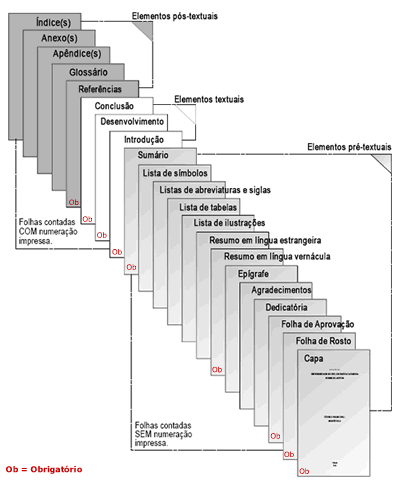
\includegraphics[width=0.3\textwidth]{./04-figuras/abnt.png}
    \caption{Exemplo de figura}
    \label{fig:abnt}
\end{figure}
\vspace*{-1,5cm}
{\raggedright \fonte{Disponível em: <https://www.gazetadopovo.com.br/abntemfoco>. Acesso em: 24 de jan. de 2015.}}
\newpage

Os títulos devem ser colocados acima das figuras. No texto devem
ser indicados pela palavra Figura acompanhada do número de ordem. E abaixo deve ser indicada sua fonte.

\section{QUADROS}

Denomina-se quadro a apresentação de dados de forma organizada, para cuja compreensão não seria necessário qualquer elaboração matemático-estatística. A identificação se fará com o nome do elemento Quadro por extenso, seguido do número de ordem em algarismo arábico. Outros elementos do quadro deverão ser descritos de acordo com o padrão usado para
Apresentação tabular.

\begin{quadro}[H]

	\begin{center}
	\caption{Exemplo para quadro.\label{qua:quaexe}}
		\begin{tabular}{|p{7cm}|p{7cm}|}
			\hline
			("Trabalho Conclusão de Curso")\\
			\hline
		\end{tabular}
	\end{center}
	\vspace*{-0,8cm}

	{\raggedright \fonte{Autor desta monografia, 2015.}}
	
\end{quadro}


\section{TABELAS}

Tabelas são conjuntos de dados numéricos, associados a um
fenômeno, dispostos numa determinada ordem da classificação. Expressam as variações qualitativas e quantitativas de um fenômeno. A finalidade básica da tabela é resumir ou sintetizar dados de maneira a fornecer o máximo de informações num mínimo de espaço.

Na apresentação de uma tabela devem ser levados em consideração
os alguns critérios. Toda tabela deve ter significado próprio, dispensando consultas ao texto. A tabela deve ser colocada em posição vertical, para facilitar a leitura dos dados. No caso em que isso seja impossível, deve ser colocada em posição horizontal, com o título voltado para a margem esquerda da folha.

Se a tabela ou quadro não couber em uma página, deve ser
continuado na página seguinte. Neste caso o final não será delimitado por traço horizontal na parte inferior e o cabeçalho será repetido na página seguinte. No texto devem ser indicadas pela palavra Tabela acompanhada do número de ordem em algarismo arábico.

\begin{table}[H]
    \centering
    \caption[Exemplo tabela]{Exemplo tabela.\label{tab:exetab}}
    \begin{tabular}{lllll}
\cline{1-4}
\multicolumn{1}{|l|}{aqqqqq} & \multicolumn{1}{l|}{qqqqqqq} & \multicolumn{1}{l|}{qqqqqqqqq} & \multicolumn{1}{l|}{} &  \\ \cline{1-4}
\multicolumn{1}{|c|}{1}      & \multicolumn{1}{c|}{3}       & \multicolumn{1}{c|}{3}         & \multicolumn{1}{l|}{} &  \\ \cline{1-4}
                             &                              &                                &                       &  \\
                             &                              &                                &                       & 
\end{tabular}
\end{table}
\vspace*{-0,9cm}
{\raggedright \fonte{Autor desta monografia, 2014.}}

\section{GRÁFICOS}

Depois de sintetizados em tabelas, os dados podem ser
apresentados em gráficos, com a finalidade de proporcionar ao interessado uma visão rápida do comportamento do fenômeno. Serve para representar qualquer tabela de maneira simples, legível e interessante, tornando claros os fatos que poderiam passar despercebidos em dados apenas tabulados.

O elemento de identificação ordenado do gráfico, ou seja, o
número de ordem do mesmo no trabalho. No texto devem ser indicados pela palavra Gráfico, acompanhada do número de ordem em algarismo arábico.
